\newpage
\section{Resultados e discussões}
\subsection{Transformação genética de \textit{Escherichia coli} com proteínas
fluorescentes}
\begin{wrapfigure}{l}{0.35\textwidth}
    \centering
    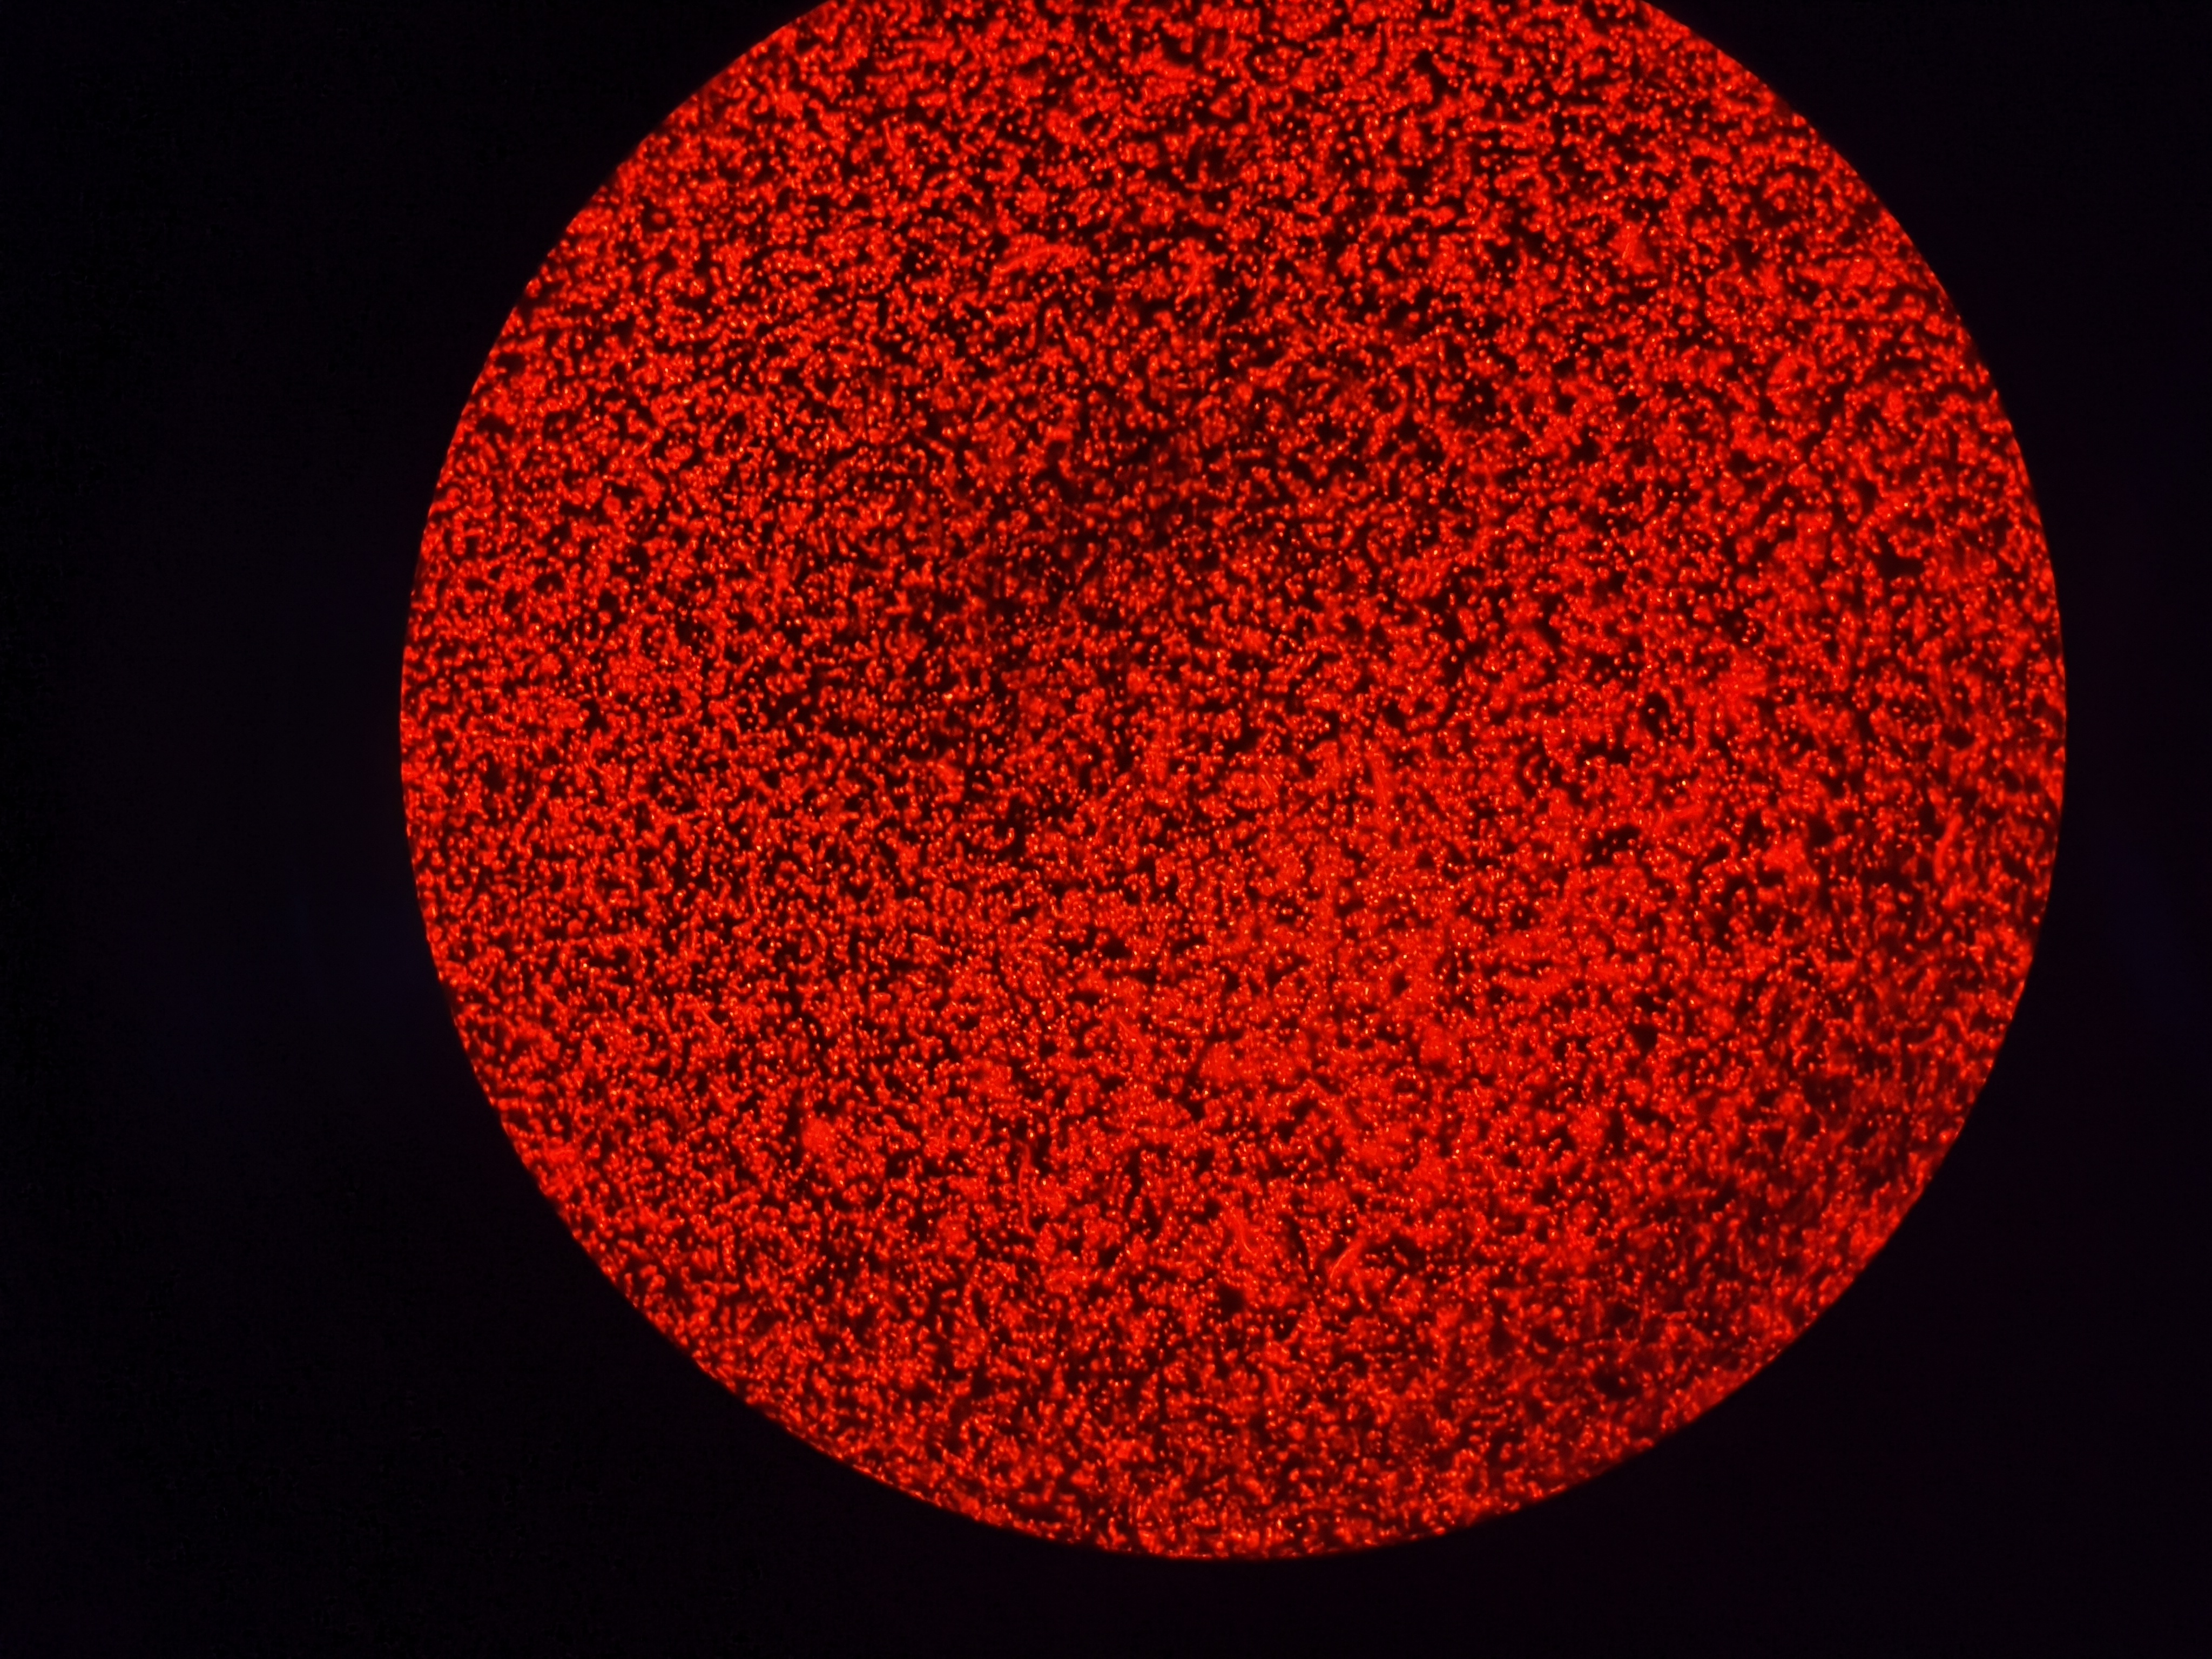
\includegraphics[width=.30\textwidth]{fig/red.jpg}
    \caption{Microscopia de fluorescência de \textit{Escherichia coli}
    transformada com plasmídeo contendo mCherry. Imagem retirada direto da lente
    ocular do microscópio.}
    \label{mCherry}
\end{wrapfigure}
Dentre os três plasmídeos testados, observou-se crescimento
bacteriano positivo em dois casos: (i) as colônias transformadas com o plasmídeo
contendo mCherry exibiram coloração vermelha característica, e (ii) as colônias
transformadas com mTAGbfp2 apresentaram fluorescência azul, conforme evidenciado
pelas imagens de microscopia de fluorescência. Veja a \cref{mCherry} e a
\cref{mTAG}.

\begin{wrapfigure}[11]{r}{0.35\textwidth}
    \centering
    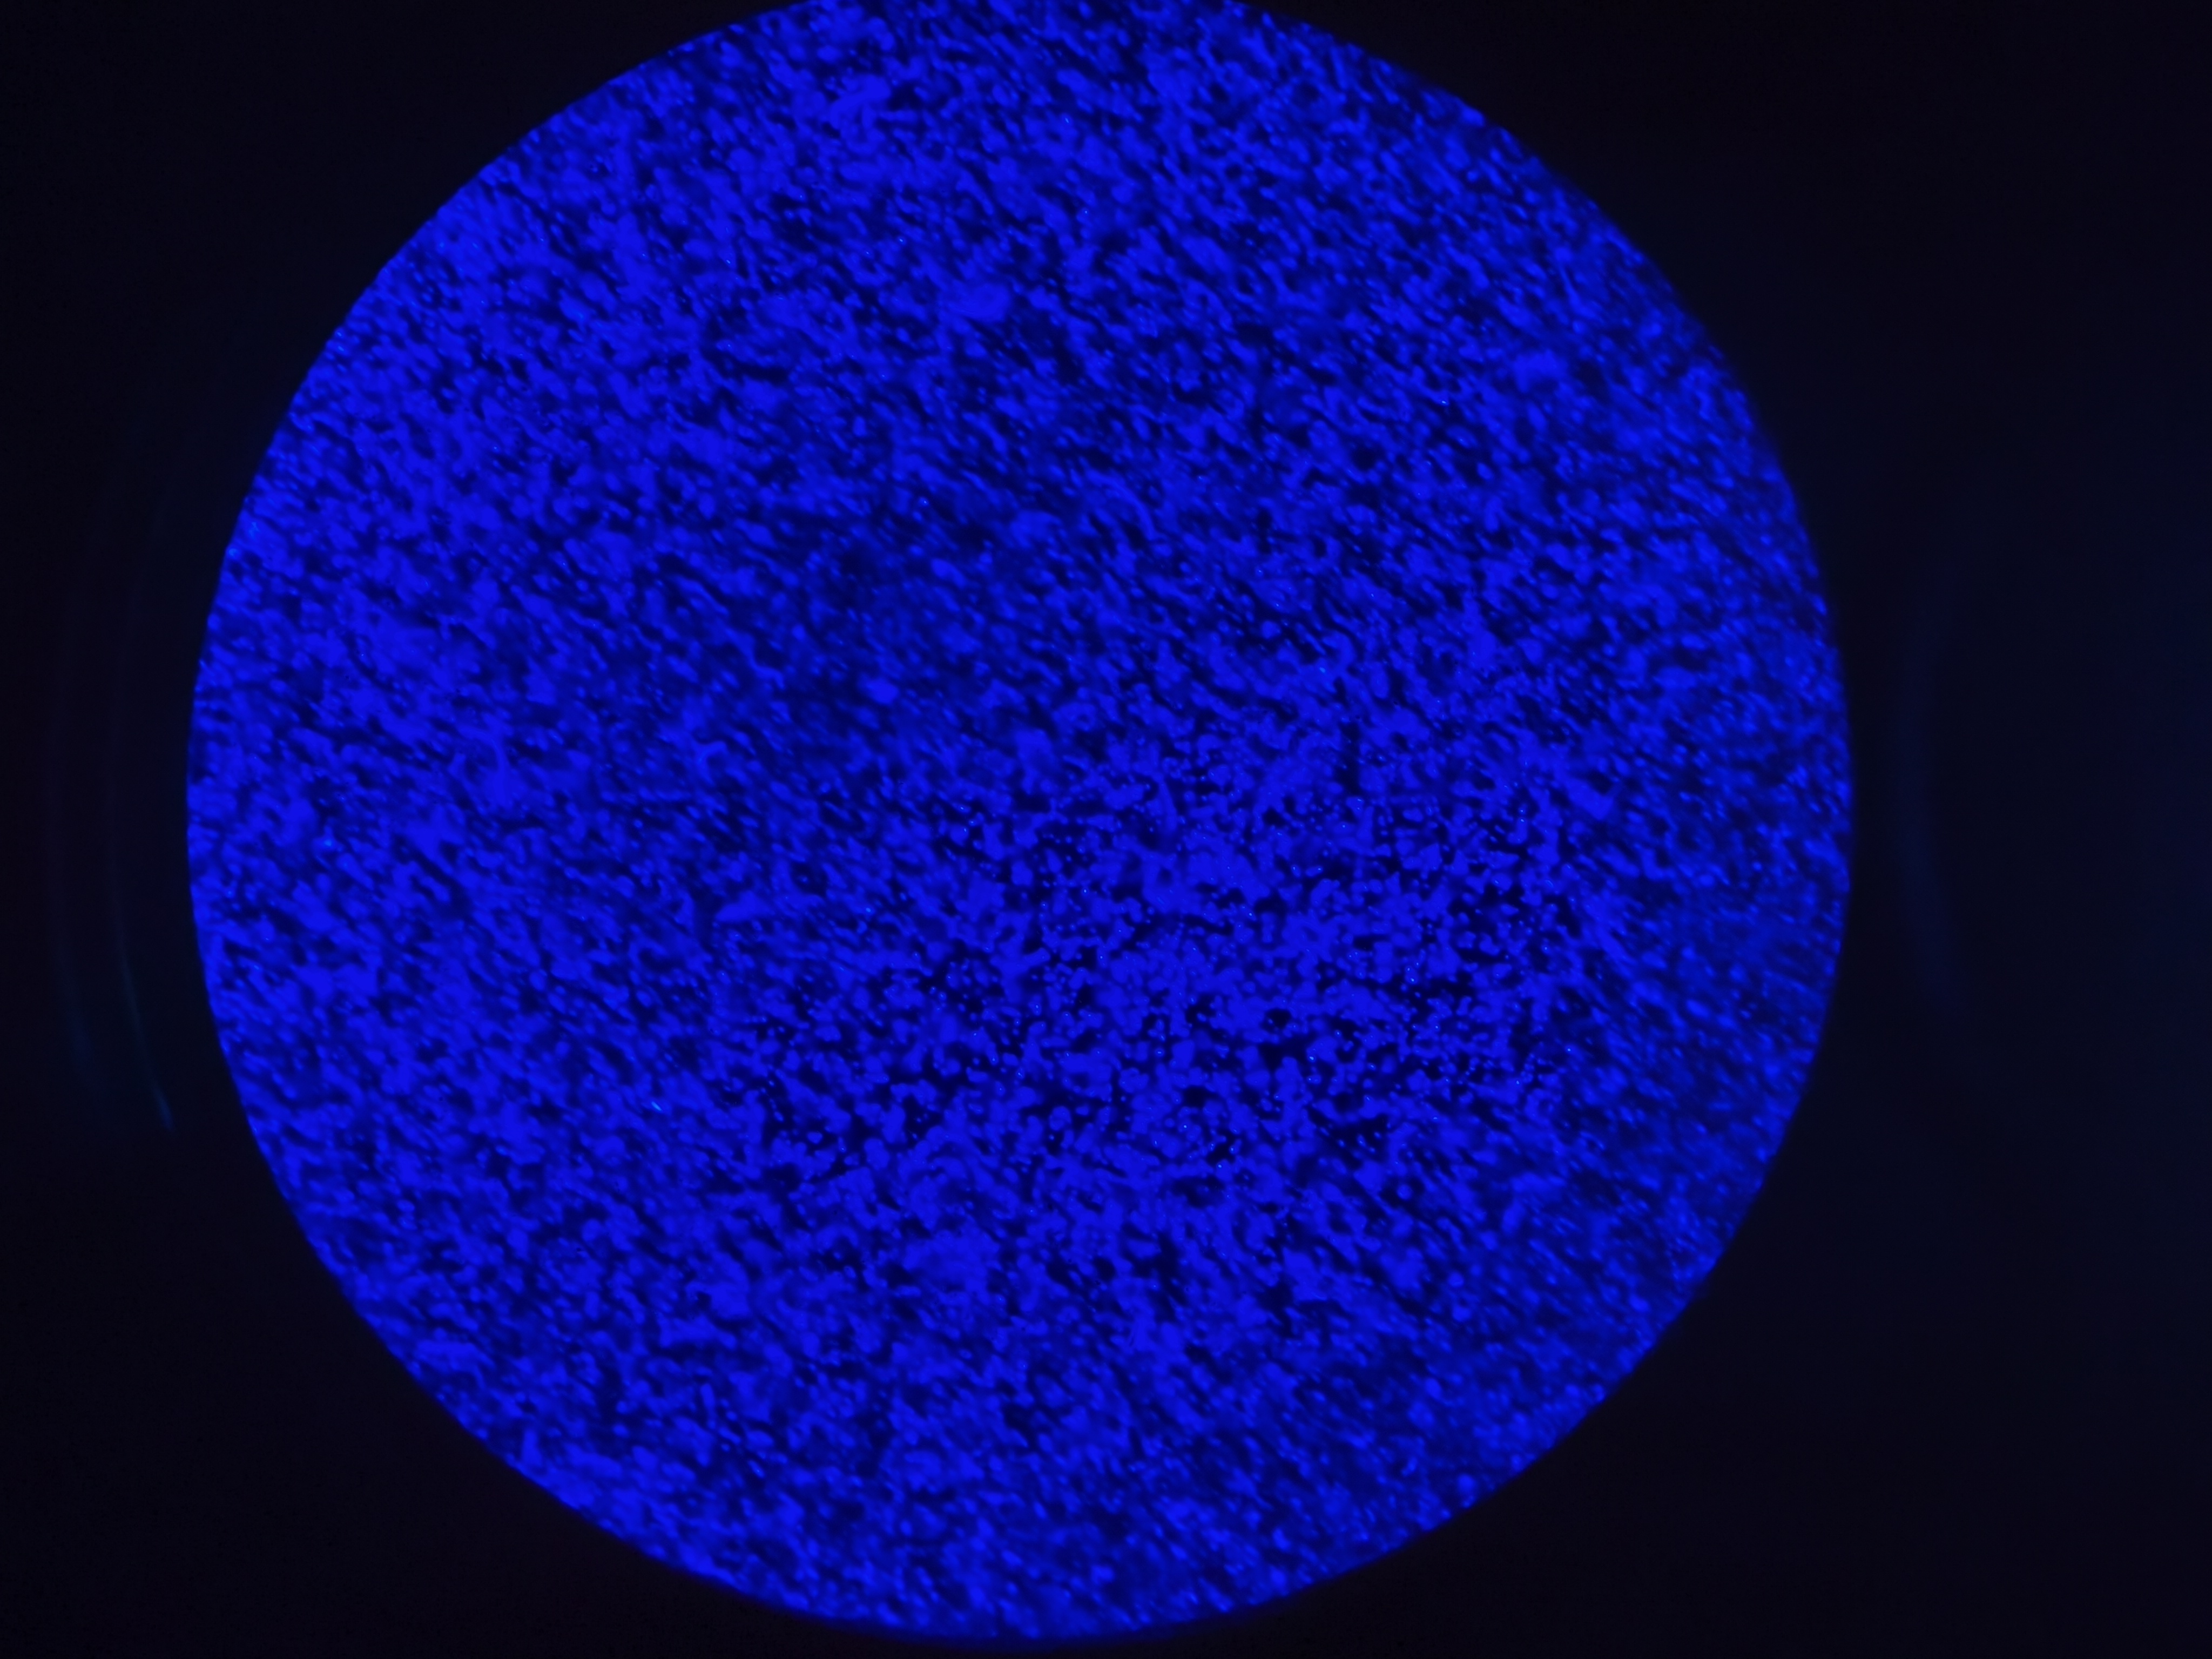
\includegraphics[width=.30\textwidth]{fig/blue.jpg}
    \caption{Microscopia de fluorescência de \textit{Escherichia coli}
    transformada com plasmídeo contendo mTAGbfp2. Imagem retirada direto da lente
    ocular do microscópio.}
    \label{mTAG}
\end{wrapfigure}

Em contraste, a transformação com o plasmídeo contendo GFP não resultou em
colônias viáveis, indicando falha nesse caso específico. Uma análise posterior
revelou que essa falha estava associada à baixa concentração do plasmídeo
durante a transformação, possivelmente devido à quantidade limitada disponível.
Esse fator técnico pode ter comprometido a eficiência da transformação,
explicando a ausência de crescimento bacteriano nessa condição.

Por fim, a correlação entre as cores observadas na transformações bem-sucedidas
e os marcadores genéticos esperados confirma a especificidade dos resultados
obtidos.

\subsection{Transformação genética de plantas por meio de Agroinfiltração (\textit{Agrobacterium tumefaciens})}
Os procedimentos de transformação das plantas \textit{Nicotiana benthamiana}, \textit{Nicotiana tabacum} e \textit{Solanum lycopersicum} via \textit{Agrobacterium spp.} foram executados conforme descrito nos métodos. Porém, os resultados mostraram viração significativa na eficiência de transformação entre as espécies, sendo observada expressão minimamente significativas apenas na \textit{Solanum lycopersicum}.
Nas \textit{N. benthamiana} e \textit{N. tabacum}, a fluorescencia associada á expressão do transgene não foi detectada de forma alguma. Já na \textit{S. lycopersicum}, embora a expressão também não tenha sido extremamente significativa, foi possível observar-se regiões com fluorescência pontuais como mostrado na figura ??, indicando uma resposta mais eficiente à agroinfiltração.

Essa diferença na eficiência da transformação e, principalmente, a completa falta de expressão nas epécies de \textit{Nicotiana}, podem estar relacionadas a diversos fatores, como a escolha errônea da área seccionada e sua orientação, falta de experiência dos grupos em realizar tais cortes e o pouco tempo que as plantas ficaram na casa de vegetação, já que ficaram apenas dois dias e o período ideal era de três a cinco dias, e até uma maior resistência à infeccção por \textit{Agrobacterium} nas espécies de \textit{Nicotiniana} o que fez com que a infecção possívelmente ainda não tivesse ocorrido da melhor forma. Dessa forma, estudos adicionais são necessários para otimizar o protocolo visando maior eficiência, particularmente nas espécies de \textit{Nicotiana}, que apresetaram baixa resposta sob as condições testadas. 
